\begin{figure}
	\centering
	\pgfplotsset{every axis legend/.append style={
		at={(1.05,0.5)},
		anchor=west}}
	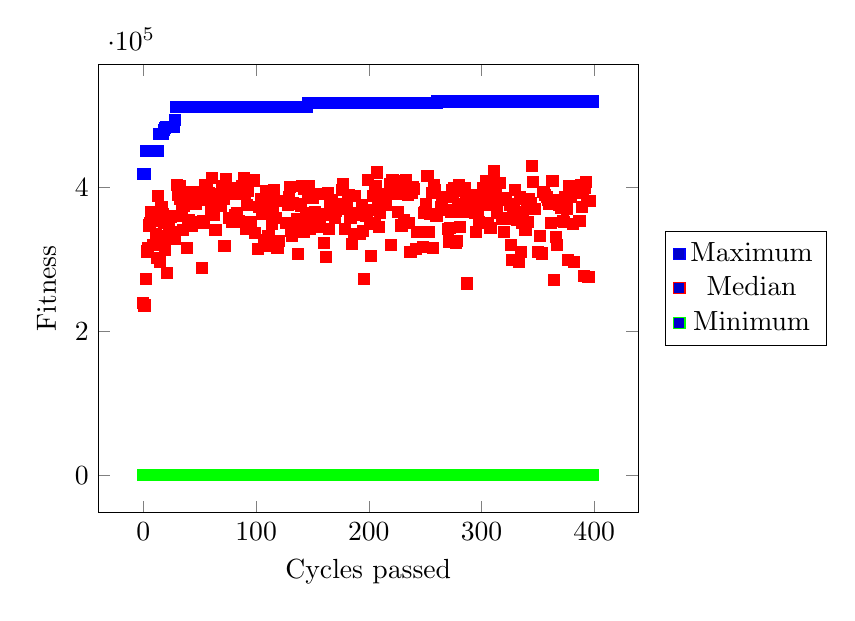
\begin{tikzpicture}
		\begin{axis}[
			xlabel=Cycles passed,
			ylabel=Fitness,
			scatter/classes={
				max={mark=square*,blue},
				med={mark=square*,red},
				min={mark=square*,green}
				}
            ]
            
\addplot+[scatter,only marks,scatter src=explicit symbolic]table[meta=label] {
x y label
0 418318 max
1 418318 max
2 451042 max
3 451042 max
4 451042 max
5 451042 max
6 451042 max
7 451042 max
8 451042 max
9 451042 max
10 451042 max
11 451042 max
12 451042 max
13 451042 max
14 474773 max
15 474773 max
16 474773 max
17 474773 max
18 479585 max
19 482122 max
20 484499 max
21 484499 max
22 484499 max
23 484499 max
24 484499 max
25 484499 max
26 484499 max
27 484499 max
28 494226 max
29 512351 max
30 512351 max
31 512351 max
32 512351 max
33 512351 max
34 512351 max
35 512351 max
36 512351 max
37 512351 max
38 512351 max
39 512351 max
40 512351 max
41 512351 max
42 512351 max
43 512351 max
44 512351 max
45 512351 max
46 512351 max
47 512351 max
48 512351 max
49 512351 max
50 512351 max
51 512351 max
52 512351 max
53 512351 max
54 512351 max
55 512351 max
56 512351 max
57 512351 max
58 512351 max
59 512351 max
60 512351 max
61 512351 max
62 512351 max
63 512351 max
64 512351 max
65 512351 max
66 512351 max
67 512351 max
68 512351 max
69 512351 max
70 512351 max
71 512351 max
72 512351 max
73 512351 max
74 512351 max
75 512351 max
76 512351 max
77 512351 max
78 512351 max
79 512351 max
80 512351 max
81 512351 max
82 512351 max
83 512351 max
84 512351 max
85 512351 max
86 512351 max
87 512351 max
88 512351 max
89 512351 max
90 512351 max
91 512351 max
92 512351 max
93 512351 max
94 512351 max
95 512351 max
96 512351 max
97 512351 max
98 512351 max
99 512351 max
100 512351 max
101 512351 max
102 512351 max
103 512351 max
104 512351 max
105 512351 max
106 512351 max
107 512351 max
108 512351 max
109 512351 max
110 512351 max
111 512351 max
112 512351 max
113 512351 max
114 512351 max
115 512351 max
116 512351 max
117 512351 max
118 512351 max
119 512351 max
120 512351 max
121 512351 max
122 512351 max
123 512351 max
124 512351 max
125 512351 max
126 512351 max
127 512351 max
128 512351 max
129 512351 max
130 512351 max
131 512351 max
132 512351 max
133 512351 max
134 512351 max
135 512351 max
136 512351 max
137 512351 max
138 512351 max
139 512351 max
140 512351 max
141 512351 max
142 512351 max
143 512351 max
144 512351 max
145 512351 max
146 517373 max
147 517373 max
148 517373 max
149 517373 max
150 517373 max
151 517373 max
152 517373 max
153 517373 max
154 517373 max
155 517373 max
156 517373 max
157 517373 max
158 517373 max
159 517373 max
160 517373 max
161 517373 max
162 517373 max
163 517373 max
164 517373 max
165 517373 max
166 517373 max
167 517373 max
168 517373 max
169 517373 max
170 517373 max
171 517373 max
172 517373 max
173 517373 max
174 517373 max
175 517373 max
176 517373 max
177 517373 max
178 517373 max
179 517373 max
180 517373 max
181 517373 max
182 517373 max
183 517373 max
184 517373 max
185 517373 max
186 517373 max
187 517373 max
188 517373 max
189 517373 max
190 517373 max
191 517373 max
192 517373 max
193 517373 max
194 517373 max
195 517373 max
196 517373 max
197 517373 max
198 517373 max
199 517373 max
200 517373 max
201 517373 max
202 517373 max
203 517373 max
204 517373 max
205 517373 max
206 517373 max
207 517373 max
208 517373 max
209 517373 max
210 517373 max
211 517373 max
212 517373 max
213 517373 max
214 517373 max
215 517373 max
216 517373 max
217 517373 max
218 517373 max
219 517373 max
220 517373 max
221 517373 max
222 517373 max
223 517373 max
224 517373 max
225 517373 max
226 517373 max
227 517373 max
228 517373 max
229 517373 max
230 517373 max
231 517373 max
232 517373 max
233 517373 max
234 517373 max
235 517373 max
236 517373 max
237 517373 max
238 517373 max
239 517373 max
240 517373 max
241 517373 max
242 517373 max
243 517373 max
244 517373 max
245 517373 max
246 517373 max
247 517373 max
248 517373 max
249 517373 max
250 517373 max
251 517373 max
252 517373 max
253 517373 max
254 517373 max
255 517373 max
256 517373 max
257 517373 max
258 517373 max
259 517373 max
260 517373 max
261 519450 max
262 519450 max
263 519450 max
264 519450 max
265 519450 max
266 519450 max
267 519450 max
268 519450 max
269 519450 max
270 519450 max
271 519450 max
272 519450 max
273 519450 max
274 519450 max
275 519450 max
276 519450 max
277 519450 max
278 519450 max
279 519450 max
280 519450 max
281 519450 max
282 519450 max
283 519450 max
284 519450 max
285 519450 max
286 519450 max
287 519450 max
288 519450 max
289 519450 max
290 519450 max
291 519450 max
292 519450 max
293 519450 max
294 519450 max
295 519450 max
296 519450 max
297 519450 max
298 519450 max
299 519450 max
300 519450 max
301 519450 max
302 519450 max
303 519450 max
304 519450 max
305 519450 max
306 519450 max
307 519450 max
308 519450 max
309 519450 max
310 519450 max
311 519450 max
312 519450 max
313 519450 max
314 519450 max
315 519450 max
316 519450 max
317 519450 max
318 519450 max
319 519450 max
320 519450 max
321 519450 max
322 519450 max
323 519450 max
324 519450 max
325 519450 max
326 519450 max
327 519450 max
328 519450 max
329 519450 max
330 519450 max
331 519450 max
332 519450 max
333 519450 max
334 519450 max
335 519450 max
336 519450 max
337 519450 max
338 519450 max
339 519450 max
340 519450 max
341 519450 max
342 519450 max
343 519450 max
344 519450 max
345 519450 max
346 519450 max
347 519450 max
348 519450 max
349 519450 max
350 519450 max
351 519450 max
352 519450 max
353 519450 max
354 519450 max
355 519450 max
356 519450 max
357 519450 max
358 519450 max
359 519450 max
360 519450 max
361 519450 max
362 519450 max
363 519450 max
364 519450 max
365 519450 max
366 519450 max
367 519450 max
368 519450 max
369 519450 max
370 519450 max
371 519450 max
372 519450 max
373 519450 max
374 519450 max
375 519450 max
376 519450 max
377 519450 max
378 519450 max
379 519450 max
380 519450 max
381 519450 max
382 519450 max
383 519450 max
384 519450 max
385 519450 max
386 519450 max
387 519450 max
388 519450 max
389 519450 max
390 519450 max
391 519450 max
392 519450 max
393 519450 max
394 519450 max
395 519450 max
396 519450 max
397 519450 max
398 519450 max
399 519450 max
};
\addplot+[scatter,only marks,scatter src=explicit symbolic]table[meta=label] {
x y label
0 239097 med
1 235804 med
2 272837 med
3 310884 med
4 316151 med
5 347185 med
6 350081 med
7 365861 med
8 353244 med
9 319627 med
10 361191 med
11 335571 med
12 302248 med
13 387975 med
14 325963 med
15 296754 med
16 372259 med
17 363654 med
18 351233 med
19 313382 med
20 332682 med
21 281230 med
22 328743 med
23 345530 med
24 359712 med
25 0 med
26 338517 med
27 0 med
28 328891 med
29 360891 med
30 403797 med
31 389605 med
32 401260 med
33 384204 med
34 371640 med
35 340875 med
36 374785 med
37 389827 med
38 0 med
39 316401 med
40 355133 med
41 384404 med
42 393869 med
43 346331 med
44 350473 med
45 391619 med
46 352524 med
47 377196 med
48 393003 med
49 0 med
50 0 med
51 391440 med
52 288583 med
53 353795 med
54 350133 med
55 403285 med
56 401673 med
57 382316 med
58 392689 med
59 386390 med
60 366043 med
61 412730 med
62 390147 med
63 361884 med
64 341127 med
65 373793 med
66 391254 med
67 377359 med
68 0 med
69 374946 med
70 401803 med
71 384045 med
72 318587 med
73 411533 med
74 395604 med
75 0 med
76 357913 med
77 0 med
78 399499 med
79 351571 med
80 393217 med
81 362200 med
82 391426 med
83 364099 med
84 392842 med
85 352639 med
86 0 med
87 391942 med
88 401616 med
89 412397 med
90 391665 med
91 342763 med
92 375271 med
93 395033 med
94 346264 med
95 352404 med
96 0 med
97 0 med
98 409638 med
99 336807 med
100 0 med
101 0 med
102 313974 med
103 372506 med
104 384130 med
105 362635 med
106 373063 med
107 322703 med
108 0 med
109 394752 med
110 326958 med
111 332397 med
112 318810 med
113 379032 med
114 349822 med
115 367760 med
116 396272 med
117 0 med
118 358075 med
119 315454 med
120 325049 med
121 381639 med
122 0 med
123 0 med
124 0 med
125 0 med
126 0 med
127 350540 med
128 375577 med
129 386202 med
130 400979 med
131 339544 med
132 333335 med
133 378233 med
134 338876 med
135 0 med
136 356638 med
137 307273 med
138 0 med
139 377396 med
140 374142 med
141 402481 med
142 337523 med
143 397392 med
144 365039 med
145 352052 med
146 389734 med
147 402084 med
148 342394 med
149 348439 med
150 385394 med
151 350538 med
152 366001 med
153 0 med
154 0 med
155 0 med
156 362453 med
157 344586 med
158 390425 med
159 0 med
160 323165 med
161 0 med
162 303852 med
163 361917 med
164 391875 med
165 342514 med
166 377579 med
167 383022 med
168 0 med
169 374626 med
170 357000 med
171 367218 med
172 377048 med
173 0 med
174 371804 med
175 376787 med
176 396568 med
177 405235 med
178 0 med
179 342172 med
180 370701 med
181 373379 med
182 389720 med
183 357320 med
184 358121 med
185 321821 med
186 364536 med
187 335589 med
188 388281 med
189 0 med
190 0 med
191 0 med
192 335058 med
193 362392 med
194 375992 med
195 339274 med
196 273306 med
197 0 med
198 361038 med
199 410431 med
200 0 med
201 350445 med
202 304482 med
203 368835 med
204 387799 med
205 348973 med
206 401903 med
207 420928 med
208 380555 med
209 344708 med
210 364363 med
211 0 med
212 378922 med
213 0 med
214 390233 med
215 376339 med
216 0 med
217 0 med
218 0 med
219 404008 med
220 320053 med
221 410627 med
222 408673 med
223 0 med
224 394778 med
225 391092 med
226 366368 med
227 406512 med
228 397300 med
229 347129 med
230 0 med
231 354964 med
232 393523 med
233 410073 med
234 0 med
235 390309 med
236 350361 med
237 309961 med
238 393095 med
239 399924 med
240 398131 med
241 0 med
242 314039 med
243 337516 med
244 0 med
245 0 med
246 0 med
247 0 med
248 316903 med
249 364331 med
250 365224 med
251 377391 med
252 416421 med
253 338463 med
254 362842 med
255 362961 med
256 392162 med
257 315516 med
258 403949 med
259 395876 med
260 360441 med
261 0 med
262 0 med
263 0 med
264 373100 med
265 377649 med
266 0 med
267 369165 med
268 368131 med
269 386559 med
270 341799 med
271 324990 med
272 343750 med
273 366387 med
274 396148 med
275 394276 med
276 398727 med
277 322469 med
278 326108 med
279 377306 med
280 403219 med
281 344909 med
282 375542 med
283 365574 med
284 395435 med
285 398483 med
286 380499 med
287 266437 med
288 365712 med
289 389148 med
290 381684 med
291 0 med
292 373083 med
293 384401 med
294 363994 med
295 338158 med
296 0 med
297 364186 med
298 352087 med
299 388736 med
300 389877 med
301 399442 med
302 377495 med
303 379319 med
304 408508 med
305 376317 med
306 351158 med
307 375312 med
308 343474 med
309 382874 med
310 407600 med
311 422579 med
312 397273 med
313 395194 med
314 365173 med
315 382621 med
316 406477 med
317 0 med
318 355613 med
319 385083 med
320 337564 med
321 356860 med
322 382640 med
323 0 med
324 0 med
325 376349 med
326 319924 med
327 299036 med
328 368831 med
329 376390 med
330 396832 med
331 366066 med
332 355378 med
333 297034 med
334 387064 med
335 309878 med
336 350467 med
337 366400 med
338 383987 med
339 340624 med
340 371195 med
341 352418 med
342 383965 med
343 0 med
344 377691 med
345 429821 med
346 407172 med
347 369955 med
348 0 med
349 0 med
350 310443 med
351 0 med
352 332904 med
353 0 med
354 308117 med
355 394013 med
356 389794 med
357 0 med
358 386976 med
359 383120 med
360 377110 med
361 378705 med
362 350039 med
363 409184 med
364 271618 med
365 382001 med
366 331341 med
367 319466 med
368 0 med
369 376011 med
370 0 med
371 371905 med
372 353739 med
373 352339 med
374 386492 med
375 0 med
376 369547 med
377 298598 med
378 401855 med
379 386534 med
380 0 med
381 349314 med
382 296181 med
383 399261 med
384 392325 med
385 402528 med
386 0 med
387 353130 med
388 403752 med
389 372736 med
390 393380 med
391 276695 med
392 399627 med
393 407071 med
394 381431 med
395 275823 med
396 380952 med
397 0 med
398 0 med
399 0 med
};
\addplot+[scatter,only marks,scatter src=explicit symbolic]table[meta=label] {
x y label
0 0 min
1 0 min
2 0 min
3 0 min
4 0 min
5 0 min
6 0 min
7 0 min
8 0 min
9 0 min
10 0 min
11 0 min
12 0 min
13 0 min
14 0 min
15 0 min
16 0 min
17 0 min
18 0 min
19 0 min
20 0 min
21 0 min
22 0 min
23 0 min
24 0 min
25 0 min
26 0 min
27 0 min
28 0 min
29 0 min
30 0 min
31 0 min
32 0 min
33 0 min
34 0 min
35 0 min
36 0 min
37 0 min
38 0 min
39 0 min
40 0 min
41 0 min
42 0 min
43 0 min
44 0 min
45 0 min
46 0 min
47 0 min
48 0 min
49 0 min
50 0 min
51 0 min
52 0 min
53 0 min
54 0 min
55 0 min
56 0 min
57 0 min
58 0 min
59 0 min
60 0 min
61 0 min
62 0 min
63 0 min
64 0 min
65 0 min
66 0 min
67 0 min
68 0 min
69 0 min
70 0 min
71 0 min
72 0 min
73 0 min
74 0 min
75 0 min
76 0 min
77 0 min
78 0 min
79 0 min
80 0 min
81 0 min
82 0 min
83 0 min
84 0 min
85 0 min
86 0 min
87 0 min
88 0 min
89 0 min
90 0 min
91 0 min
92 0 min
93 0 min
94 0 min
95 0 min
96 0 min
97 0 min
98 0 min
99 0 min
100 0 min
101 0 min
102 0 min
103 0 min
104 0 min
105 0 min
106 0 min
107 0 min
108 0 min
109 0 min
110 0 min
111 0 min
112 0 min
113 0 min
114 0 min
115 0 min
116 0 min
117 0 min
118 0 min
119 0 min
120 0 min
121 0 min
122 0 min
123 0 min
124 0 min
125 0 min
126 0 min
127 0 min
128 0 min
129 0 min
130 0 min
131 0 min
132 0 min
133 0 min
134 0 min
135 0 min
136 0 min
137 0 min
138 0 min
139 0 min
140 0 min
141 0 min
142 0 min
143 0 min
144 0 min
145 0 min
146 0 min
147 0 min
148 0 min
149 0 min
150 0 min
151 0 min
152 0 min
153 0 min
154 0 min
155 0 min
156 0 min
157 0 min
158 0 min
159 0 min
160 0 min
161 0 min
162 0 min
163 0 min
164 0 min
165 0 min
166 0 min
167 0 min
168 0 min
169 0 min
170 0 min
171 0 min
172 0 min
173 0 min
174 0 min
175 0 min
176 0 min
177 0 min
178 0 min
179 0 min
180 0 min
181 0 min
182 0 min
183 0 min
184 0 min
185 0 min
186 0 min
187 0 min
188 0 min
189 0 min
190 0 min
191 0 min
192 0 min
193 0 min
194 0 min
195 0 min
196 0 min
197 0 min
198 0 min
199 0 min
200 0 min
201 0 min
202 0 min
203 0 min
204 0 min
205 0 min
206 0 min
207 0 min
208 0 min
209 0 min
210 0 min
211 0 min
212 0 min
213 0 min
214 0 min
215 0 min
216 0 min
217 0 min
218 0 min
219 0 min
220 0 min
221 0 min
222 0 min
223 0 min
224 0 min
225 0 min
226 0 min
227 0 min
228 0 min
229 0 min
230 0 min
231 0 min
232 0 min
233 0 min
234 0 min
235 0 min
236 0 min
237 0 min
238 0 min
239 0 min
240 0 min
241 0 min
242 0 min
243 0 min
244 0 min
245 0 min
246 0 min
247 0 min
248 0 min
249 0 min
250 0 min
251 0 min
252 0 min
253 0 min
254 0 min
255 0 min
256 0 min
257 0 min
258 0 min
259 0 min
260 0 min
261 0 min
262 0 min
263 0 min
264 0 min
265 0 min
266 0 min
267 0 min
268 0 min
269 0 min
270 0 min
271 0 min
272 0 min
273 0 min
274 0 min
275 0 min
276 0 min
277 0 min
278 0 min
279 0 min
280 0 min
281 0 min
282 0 min
283 0 min
284 0 min
285 0 min
286 0 min
287 0 min
288 0 min
289 0 min
290 0 min
291 0 min
292 0 min
293 0 min
294 0 min
295 0 min
296 0 min
297 0 min
298 0 min
299 0 min
300 0 min
301 0 min
302 0 min
303 0 min
304 0 min
305 0 min
306 0 min
307 0 min
308 0 min
309 0 min
310 0 min
311 0 min
312 0 min
313 0 min
314 0 min
315 0 min
316 0 min
317 0 min
318 0 min
319 0 min
320 0 min
321 0 min
322 0 min
323 0 min
324 0 min
325 0 min
326 0 min
327 0 min
328 0 min
329 0 min
330 0 min
331 0 min
332 0 min
333 0 min
334 0 min
335 0 min
336 0 min
337 0 min
338 0 min
339 0 min
340 0 min
341 0 min
342 0 min
343 0 min
344 0 min
345 0 min
346 0 min
347 0 min
348 0 min
349 0 min
350 0 min
351 0 min
352 0 min
353 0 min
354 0 min
355 0 min
356 0 min
357 0 min
358 0 min
359 0 min
360 0 min
361 0 min
362 0 min
363 0 min
364 0 min
365 0 min
366 0 min
367 0 min
368 0 min
369 0 min
370 0 min
371 0 min
372 0 min
373 0 min
374 0 min
375 0 min
376 0 min
377 0 min
378 0 min
379 0 min
380 0 min
381 0 min
382 0 min
383 0 min
384 0 min
385 0 min
386 0 min
387 0 min
388 0 min
389 0 min
390 0 min
391 0 min
392 0 min
393 0 min
394 0 min
395 0 min
396 0 min
397 0 min
398 0 min
399 0 min
};

			\addlegendentry{Maximum}
			\addlegendentry{Median}
			\addlegendentry{Minimum}
		\end{axis}
	\end{tikzpicture}
	\caption{Detail of genetic algorithm on balanced data with 40 elements in set}
\label{plot:genProfile40}
\end{figure}
